\section{Introduction}\label{sec:Introduction}
Ever since experiments gained access to the quantum regime, there has been a continuing need to develop and perfect efficient techniques to manipulate quantum systems. These manipulations occur in real time, and the corresponding time-dependent control parameter can be described by a function of time, called the \textit{control protocol}. The recent development of quantum-enhanced devices has led to a significant surge in activity which has witnessed some remarkable advances, both theoretical and experimental, in the use of these control techniques; for example quantum control has found fertile application in assessing the thermodynamics of quantum systems, providing a means to boost the performance of nanoscale quantum heat engines, to develop ultraprecise quantum sensors, and to robustly implement quantum gates~\cite{Koch2022, STAreview}. 

Unlike classical mechanics, where the most common way of achieving control is to apply mechanical forces, in quantum control electromagnetic fields prevail, both in the DC and the AC regime. This can be traced back to the necessity to couple to Angstrom-sized atoms, and even smaller objects, where quantum effects become prevalent. Moving beyond the control of a single system to few and multi-particle settings introduces other control knobs besides external potentials, in particular, varying the interaction strength. For instance, in ultracold atoms this can be achieved using so-called Feshbach resonances~\cite{bloch2008manybody}, while in systems of optical tweezer arrays, one can directly control the positions of the trapped atoms which effectively fine-tunes the strength of the position-dependent interaction potential~\cite{Kaufman2021}. The ability to manipulate an arbitrary quantum system then becomes a multifaceted problem, one which must also be cognisant of other physically relevant constraints, for example: a finite control pulse energy and/or bandwidth, smoothness of the control protocol, or the intrinsic decoherence time which will bound the protocol time duration that can vary greatly between different physical platforms~\cite{Koch2022, STAreview, PRXQtutorial, baldwin2021optimal}. These constraints can feed directly into characterising the efficacy of a control protocol with the most common figure of merit being the fidelity (quantum overlap), between the protocol-evolved final state, $\ket{\psi(t)}$ and the desired target state, $\ket{\psi_*}$, 
\begin{equation}
\label{Eq1Fidelity}
\mathcal{F} = \vert \bra{\psi_*} \psi(t)\rangle \vert^2
\end{equation}
where we have assumed the states in Eq.~\eqref{Eq1Fidelity} are pure (as will be the case for all examples in this tutorial); however, we remark that these states could also be eigenstates or mixed ensembles. 
%Depending on the protocol duration, it may or may not be possible to reach the target state with unit fidelity. The minimum duration required to reach strictly unit fidelity is known as the quantum speed limit~\cite{mandelstam1945,fleming1973unitarity,bhattacharyya1983quantum} ~\ciref. 
While we will focus on the use of fidelity as our key figure of merit throughout this tutorial, it is important to note that when it comes to many-body states this should be done with care since it often decreases exponentially with the number of particles. Indeed, if we consider a product state with single particle fidelity of $0.99$, the many-body fidelity of a system with $100$ particles is $0.99^{100}\approx 0.36\ll 0.99$. In general there are many possible cost functions that can be used when optimising the dynamics of a quantum system, for example, the energy (density) is typically minimized in the process of preparing the ground state of a quantum system. More generally, one might be interested in maximizing and/or minimizing the expectation values of a specific observable, e.g., the magnetization, the momentum distribution, the strength of a correlation function or less frequently accessible quantities, such as quantum entanglement~\cite{kraus2001optimal,goerz2011,watts2015optimizing,tashev2024reinforcement}.  Regardless of the specific choice, the techniques presented below can be readily adapted for a given situation.

In large, spatially extended systems, it is often useful to consider two kinds of control protocols: global and local. Global protocols usually act (almost) homogeneously on the entire system, while local protocols can either be applied to a smaller part of the system or to individual constituents, e.g., the atoms of a chain using single-site addressability. Whatever the means of controlling a quantum system, it is important to keep in mind that the control protocols that can be emulated in experiments typically correspond to local (or sums of local) operators in the Hamiltonian description of the system; this is particularly relevant for many-body control. Thus, locality imposes a formidable, yet very physical, constraint on the accessibility of control fields~\cite{bukov2019geometric}. The various control techniques that are known to be effective for single, isolated quantum systems must be carefully analyzed in view of this constraint when the system size is scaled up. Providing an introduction to the tools and techniques necessary to understand the interplay between implementability and scalability of control protocols for quantum systems is the focus of this tutorial. 

%\clearpage

\begin{center}
{\bf Scope of this tutorial}
\end{center}
We aim to provide a succinct entry point to some of the state-of-the-art approaches to controlling quantum systems. There are many excellent reviews available on these and related topics, see for example Refs~\cite{Deffner2017, Glaser2015, Koch2022, STAreview, Stefanatos2020, PRXQtutorial, GiannelliPLA, Hatomura2024, ansel2024_arxiv, deffner2020thermodynamic}, which the interested reader can delve into. Here, we aim to achieve two goals: Firstly, to provide a highly pedagogical introduction to the most prevalent techniques used to control many-body systems; thus, in addition to the technical details of the control protocols themselves, we also provide extensive details on other important tools for solving paradigmatic many-body systems. Secondly, by introducing a suite of techniques arising from the various subcommunities that work on quantum control, our aim is to highlight the benefits that can arise from employing hybridized control techniques, i.e. those that take advantage of aspects of several control strategies.

With these aims in mind, in what follows we present the basic ingredients for three of the leading approaches to achieving non-adiabatic control (Fig.~\ref{fig:scope}): shortcuts-to-adiabaticity, quantum optimal control, and reinforcement learning. They are presented in isolation (and in no particular order) to ensure that the core theoretical underpinnings of each approach are presented in a suitably pedagogical manner. As such, the interested reader can dive straight into a given technique without the need to work through any preceding sections. For a given task, the choice of which approach to employ depends on a range of competing factors. The experimental architecture clearly imposes certain constraints, e.g. the available set of controls and/or measurements. Beyond such hardware limitations, however, other requirements necessarily requested from the dynamics will also impact the choice of control technique to use. For instance, if the system must follow a specific dynamical path in Hilbert space, e.g. remaining in the ground state, then the suite of tools from shortcuts-to-adiabaticity are likely to be the most suitable choice. However, in many situations the intermediate dynamics is not of any particular relevance and we are only interested in e.g. state transfer or state preparation. In these cases, often the goal is simply to find a protocol that works under the given constraints and, therefore, the task becomes principally about pulse shape optimisation where optimal control provides several efficient approaches. If, on the other hand, one is interested in automating the procedure of finding optimal protocols, then adopting a deep learning approach is advisable, as it allows trained RL agents to generalize and produce control protocols even for parameter values not encountered during optimization; moreover, RL algorithms are particularly useful for on-line feedback control based on (partial) measurements. In Sec.~\ref{sec:comparison} we provide further discussion along these lines, aiming to highlight some of the strengths and weaknesses of the techniques that we discuss in this tutorial and highlight the benefit that comes from combining techniques to tackle a problem.

Another motivation for this tutorial, that we believe sets this work apart from other reviews and pedagogical resources on the topic, is to provide an ``introductory one-stop-shop'' for the various control subcommunities. To facilitate this, we explicitly demonstrate the application of all protocols for the manipulation of a single two-level quantum system, in addition to several other relevant examples. \steve{These additional examples focus on the some of most common areas to which a given technique is applied. Therefore in Sec.~\ref{sec:STA} we consider the exact and approximate control of critical many-body systems, Sec.~\ref{sec:QOC} provides examples relevant to quantum computation focussing on the implementation of gates and the generation of multipartite entanglement, while Sec.~\ref{sec:RL_theory} explores universal single-qubit state preparation and active qubit feedback control using an ancilla.} In the hope of bringing some consistency to the nomenclature, we also provide tables summarising the notation employed when introducing a given technique in Table~\ref{table:AGPsSymbols} for shortcuts-to-adiabaticity, Table~\ref{table:QOCSymbols} for optimal control, and Table~\ref{table:RLSymbols} for reinforcement learning. Finally, the reader can refer to Table~\ref{table:Abbreviations} for a list of abbreviations commonly used throughout this tutorial.
We provide Jupyter notebooks for interested readers to explore further the control techniques introduced on GitHub~\cite{github_code}.

\begin{figure}[t]
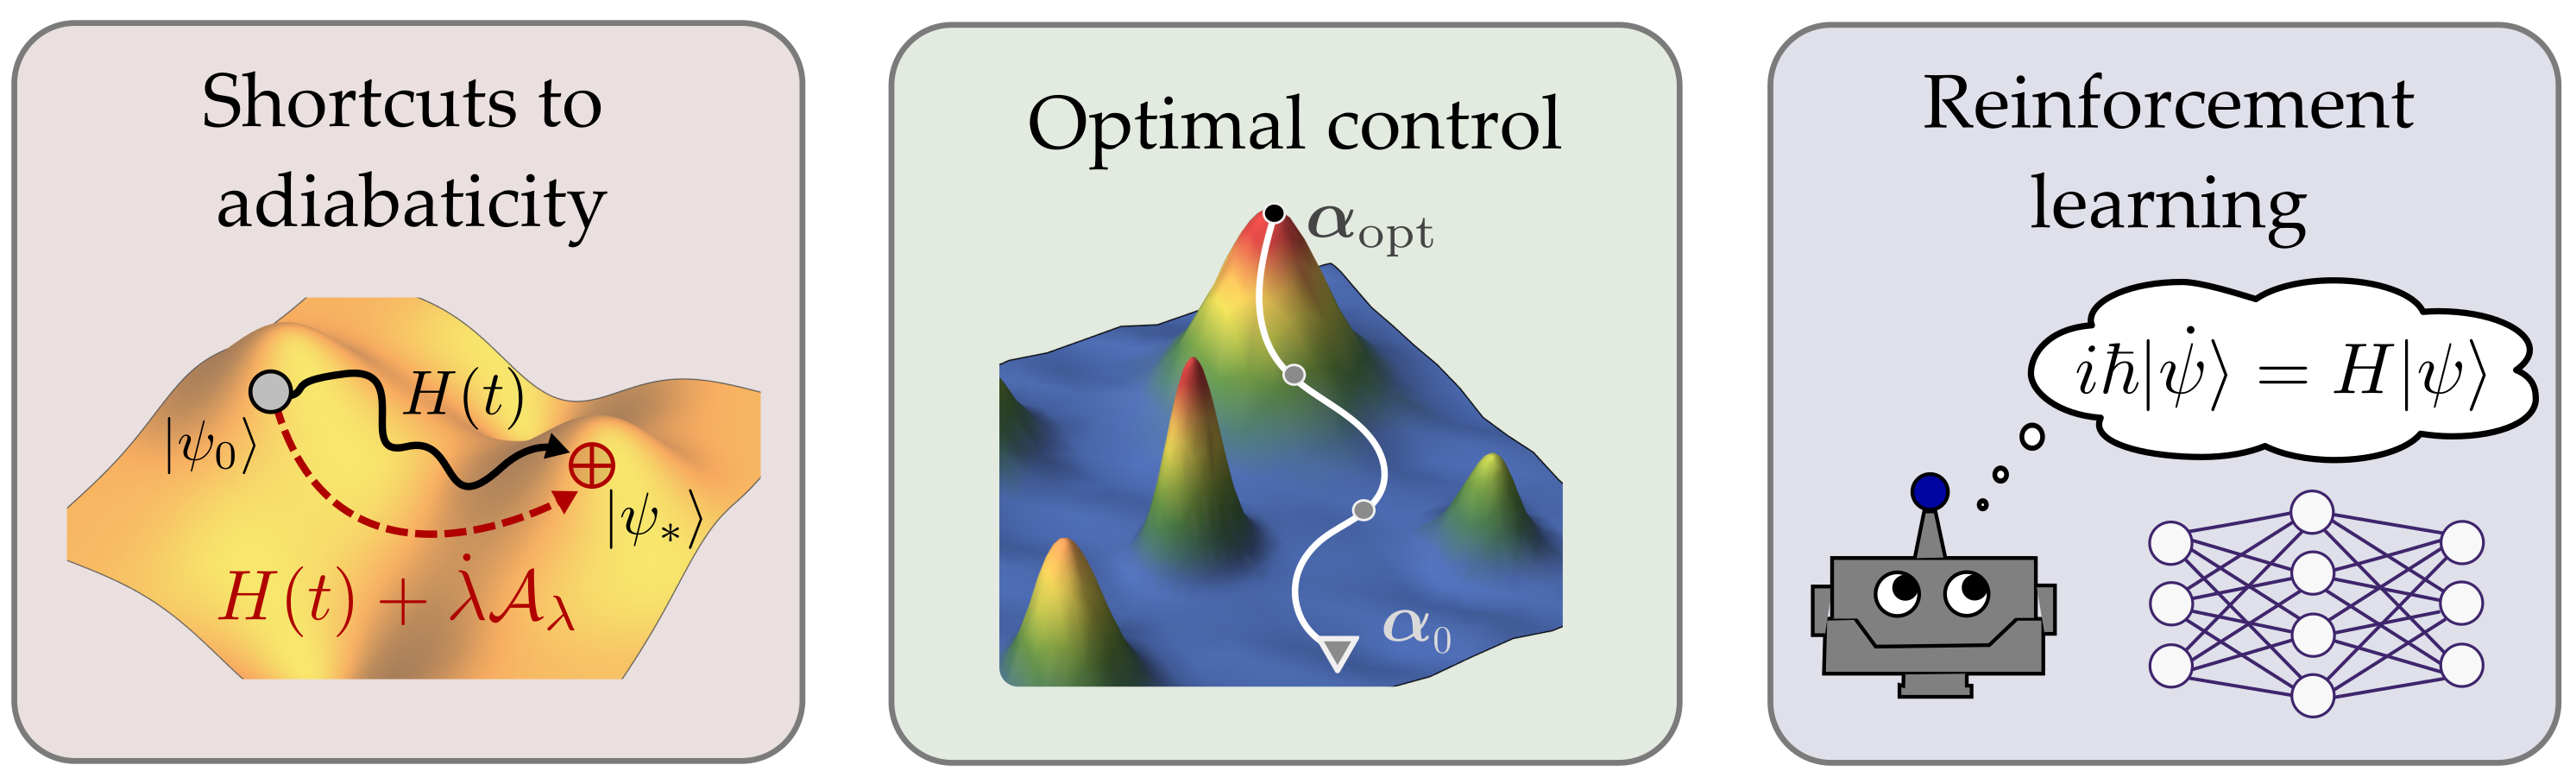
\includegraphics[width=0.9\columnwidth]{Fig_Sec1.png}
\label{fig:scope}
\caption{Schematic of the main three approaches to quantum control that are discussed in this tutorial article: shortcuts to adiabaticity (Sec. \ref{sec:STA}, optimal control (Sec. \ref{sec:QOC}), and reinforcement learning (Sec. \ref{sec:RL_theory}). }
\end{figure}

\begin{center}
{\bf METHODOLOGIES OF QUANTUM CONTROL}
\end{center}
%\label{sec:Methodologies}
We can broadly define three classes of quantum systems of increasing control complexity: Few (including single) particle systems are often used to demonstrate the basics of control methods and can also benchmark numerical quantum control algorithms against exactly solvable problems. However, they also bear relevance to real systems such as qubits (two-level systems) and qutrits or $\Lambda$-systems (three-level systems). In these settings common control problems include state population transfer or finding optimal single- or two-qubit gates. The relative simplicity of the models typically can allow for the inclusion of dissipation effects~\cite{Koch2016OpenSys}. The next class of systems that we will be primarily interested in are fermionic band models and weakly interacting bosons described by quadratic Hamiltonians. Examples in this category include topological insulators, weakly-interacting bosons, the transverse-field Ising model, and the Kitaev honeycomb model. The translation invariant counterparts of such models are exactly solvable in momentum space, which offers the possibility to explore some control techniques analytically. In particular, two-band models can be viewed as a collection of independent two-level systems labelled by (quasi)momentum. As we will demonstrate, control over the individual momentum modes allows for optimal control of the entire system, however, the momentum-dependence ultimately compromises the locality of the applied control fields in real space. Nevertheless, useful insight into the most relevant operators for achieving control can be learned which can prove valuable in moving to the final class of systems. The most complex control class comprises many-body systems with no known exact solutions, e.g., nonintegrable models with Hubbard- and Heisenberg-type Hamiltonians. In general we can expect here optimal control techniques to work whenever the state of interest is gapped in energy; for gapless models much less is known regarding their controllability, and there are many open questions at present.

Broadly speaking, we distinguish between adiabatic and non-adiabatic techniques when classifying quantum control protocols. Adiabatic protocols (which we will rigorously define for quantum systems in the proceeding sections) make use of the discrete structure of quantized spectra and high-fidelity control timescales are inversely proportional to the energy gaps of the controlled level to its neighboring levels. A famous example is the Landau-Zener model, where an exponentially small fraction is left in the excited state after the completion of the adiabatic process~\cite{LZreview}. Stimulated Rapid Adiabatic Passage (STIRAP)~\cite{STIRAPreview} is another technique which exploits spectral characteristics to achieve robust state transfer. In this tutorial, we will focus explicitly on non-adiabatic techniques. This class encompasses counter-diabatic (CD) protocols that generate a transitionless time evolution with respect to the instantaneous basis of the Hamiltonian describing the system of interest, which is typically far from the adiabatic regime. It also captures the broader set of Hamiltonians that are tailored to bring the controlled system into a target state within a fixed protocol duration (but allows for the creation of excitations during the evolution so long as they are removed before the protocol comes to an end) as is typical in many quantum optimal control approaches.\\



% \section{Methodologies of Quantum Control}
% \label{sec:Methodologies}
% We can broadly define three classes of quantum systems of increasing control complexity: Few (including single) particle systems are often used to demonstrate the basics of control methods and can also benchmark numerical quantum control algorithms against exactly solvable problems. However, they also bear relevance to real systems such as qubits (two-level systems) and qutrits or $\Lambda$-systems (three-level systems). In these settings common control problems include state population transfer or finding optimal single- or two-qubit gates. The relative simplicity of the models typically can allow for the inclusion of dissipation effects~\ciref. It is the next class of systems that we will be primarily interested in: fermionic band models and weakly interacting bosons described by quadratic Hamiltonians. Examples in this category include topological insulators, weakly-interacting bosons, the transverse-field Ising model, and the Kitaev honeycomb model. The translation invariant counterparts of such models are exactly solvable in momentum space, which offers the possibility to explore some control techniques analytically. In particular, two-band models can be viewed as a collection of independent two-level systems labelled by (quasi)momentum. As we will demonstrate, control over the individual momentum modes allows for optimal control of the entire system, however, the momentum-dependence ultimately compromises the locality of the applied control fields in real space. Nevertheless, useful insight into the most relevant operators for achieving control can be learned which can prove valuable in moving to the final class of systems. The most complex control class comprises many-body systems with no known exact solutions, e.g., nonintegrable models with Hubbard- and Heisenberg-type Hamiltonians. In general we can expect here optimal control techniques to work whenever the state of interest is gapped in energy; for gapless models much less is known regarding their controllability, and there are many open questions at present~\ciref.

% Broadly speaking, we distinguish between adiabatic and non-adiabatic techniques when classifying quantum control protocols. Adiabatic protocols (which we will rigorously define for quantum systems in the proceeding sections) make use of the discrete structure of quantized spectra and high-fidelity control timescales are inversely proportional to the energy gaps of the controlled level to its neighboring levels. Famous examples are captured by the Landau-Zener model where an exponentially small fraction is left in the excited state after the completion of the adiabatic process~\ciref and the Stimulated Rapid Adiabatic Passage technique (STIRAP)~\ciref which exploits spectral characteristics to achieve robust state transfer. In this tutorial, we will focus on explicitly on non-adiabatic techniques. This class encompasses counter-diabatic (CD) protocols~\ciref that generate a transitionless time evolution with respect to the instantaneous basis of the Hamiltonian describing the system of interest, which is typically far from the adiabatic regime. It also captures the broader set of Hamiltonians that are tailored to bring the controlled system into a target state within a fixed protocol duration (but allows for the creation of excitations during the evolution so long as they are removed before the protocol comes to an end) as is typical in many quantum optimal control approaches~\ciref.\\

% \steve{Need to segue out.}

% \begin{table}[!h]
% \centering
% \begin{tabular}{|p{12.5cm}|c|}
% \hline
% Object & Proposed Symbol \\
% \hline\hline
% Original system Hamiltonian & $H(t)$ \\
% \hline
% Berry correction (no diagonal elements, also known as Kato potential) & $\mathcal{A}_\lambda$ \\
% \hline
% Gauge potential (table point iv) [U's] & $\dot{\lambda}(i \partial_\lambda U)U^{\dagger}$ \\
% \hline
% Total generator (original system hamiltonian + controls) for Kato/Berry & $H_\text{CD}(t)=H(t) + \mathcal{A}_\lambda$ \\
% \hline
% Total generator (original system hamiltonian + controls) for AGP & $H_\text{CD}(t)=H(t) + \dot{\lambda}(i \partial_\lambda U)U^{\dagger}$ \\
% \hline
% General Gauge Potential (table point v)& ?? \\
% \hline
% Approximate AGP & $A_\lambda^{(x)}$ \\
% \hline
% Berry Connection & $\bra{n(\lambda)}\mathcal{A}_\lambda\ket{n(\lambda)}$ \\
% \hline
% Geometric and dynamical phases & $\phi_g$ and $\phi_d$ \\
% \hline
% \end{tabular}
% \end{table}

%Table of Symbols:
% \begin{table}[!h]
% \centering
% \begin{tabular}{|p{4.5cm}|c|c|c|c|}
% 	\hline
% 	Name & Steve CD-Section & Callum CD-Section  & OC Section & ML Section \\
% 	\hline\hline
% 	Annihilation/Creation operators & $a$, $a^{\dagger}$ (also $b$'s) & - & - & - \\
% 	\hline
% 	Arbitrary Function & $f(t)$ & - & - & - \\
% 	\hline
% 	Angle in Bogoluibov Trans & $\alpha$ & - & - & - \\
% 	\hline
%         Bloch sphere coordinates & - & - & - & $\theta,\varphi$ \\
%         \hline
% 	CD Hamiltonian/Berry Term & $H_{CD}(t)$ & - & - & (NB!) $H_\text{CD}(t)$  \\
% 	\hline
% 	m-ranged CD Hamiltonian Ising model term (eq.~\eqref{eq:HCDIsing2}) & $H_\text{CD}^{[m]}$ & - & - & - \\
% 	\hline
% 	Collective Spin operators & $S_\alpha = \tfrac{1}{2}\sum_n \sigma^\alpha_n$ & - & - & - \\
% 	\hline
%         Control parameters & - & - & $\bm{\alpha}$, $\alpha_i$ & - \\
%         \hline
% 	Eigenstate \& energy & $\ket{n}$, $E_n$ & - & - & - \\
% 	\hline
% 	Evolution Operator & $U(t)$ & - & $U(t)$ & $U(t,0)$ \\
% 	\hline
% 	Evolved State & $\ket{\psi(t)}$ & - & - & - \\
% 	\hline
%         Fidelity & - & - & $\mathcal{F}$ & $F$ \\
%         \hline
%         Global phase of wavefunction & - & - & - & $\alpha$ \\
%         \hline
% 	Hamiltonian & $H(t)$ & - & $H(t)$ & - \\
% 	\hline
% 	Harmonic Ocillator Freq (Eq.\eqref{eq:CDqho}) & $\omega$ & - & - & - \\
% 	\hline
%         Hilbert space dimension & - & - & $d$ & - \\
%         \hline
%         Identity operator & - & - & $\mathbb{I}$ & - \\
%         \hline
% 	Landau-Zener Model & $H=\hbar\Delta \sigma^x +  \hbar \nu(t) \sigma^z$ & - & $\hbar\Delta \sigma^x +  \hbar \nu(t) \sigma^z$ & $\Delta\sigma^z + \nu(t)\sigma^x$ \\
% 	\hline
% 	Landau-Zener Eigenstates & $\ket{\phi_g} = \cos \theta \ket{0} + \sin \theta \ket{1}$ & - & $\ket{\phi_g} \equiv \cos\left(\frac{\theta}{2}\right) \ket{0}+\sin\left(\frac{\theta}{2}\right) \ket{1}$ & - \\
% 	\hline
% 	Landau-Zener Energy gap & $\Delta$ & - & $\Delta$ & - \\
% 	\hline
% 	Landau-Zener Time Dep Field & $\nu(t)$ & - & $\nu(t)$ & - \\
% 	\hline
% 	Landau-Zener $\theta$ Parameter & $\tan \theta = -\left(\nu(t)+\sqrt{\Delta^2+\nu(t)^2}\right)/\Delta$ & - & $\tan\theta = \frac{\Delta}{\nu}$ & - \\
% 	\hline
% 	OC Cost function & - & - & $J$ & - \\ 
%         \hline
 
%         Partial Derivative & $\partial_x$ & - & $\frac{\partial}{\partial x}$ & - \\
% 	\hline
% 	Number of qubits/sites & $N$ & - & - & - \\
% 	\hline
% 	$\alpha$-Pauli Matrix on site $j$ & $\sigma^\alpha_j$ & - & - & - \\
% 	\hline
%         Pauli matrix (single qubit) & - & - & $\sigma_\alpha$ & - \\
%         \hline
% 	RL state & - & - & - &  $s$ \\
%         \hline
%         RL state space & - & - & - &  $\mathcal{S}$ \\
%         \hline
%         RL initial state probability & - & - & - &  $p(s_0)$ \\
%         \hline
%         RL action & - & - & - &  $a$ \\
%         \hline
%         RL action space & - & - & - &  $\mathcal{A}$ \\
%         \hline
%         RL reward & - & - & - &  $r(s',s',a)$ \\
%         \hline
%         RL reward space & - & - & - &  $\mathcal{R}$ \\
%         \hline
%         RL environment transition probability & - & - & - &  $p(s'|s,a)$ \\
%         \hline
%         RL episode step & - & - & - &  $t$ \\
%         \hline
%         RL, total number of episode steps & - & - & - &  $T$ \\
%         \hline
%         RL episode trajectory & - & - & - &  $\tau$ \\
%         \hline
%         RL probability for a trajectory & - & - & - &  $P_\pi(\tau)$ \\
%         \hline
%         RL, total number of trajectories & - & - & - &  $N$ \\
%         \hline
%         RL expected return & - & - & - &  $G(\tau)$ \\
%         \hline
%         RL objective & - & - & - &  $J$ \\
%         \hline
%         RL Policy  & - & - & - &  $\pi(a|s)$ \\
%         \hline
%         RL neural network parameters  & - & - & - &  $\theta$ \\
%         \hline
%         RL Q-function  & - & - & - &  $Q(s,a)$ \\
%         \hline
%         RL, gradient descent step size & - & - & - &  $\alpha$ \\
%         \hline
%         Target state & - & - & \sout{$\ket{\psi_G}$} &  $\ket{\psi_\ast}$ \\
%         \hline
%         Target unitary & - & - & \sout{$U_G$} $U_\ast$ & - \\
%         \hline
%         Time Derivative & $\dot{x}$ & - & - & - \\
% 	\hline
% 	Time Dependent Field on Ising/LMG models & $g(t)$ & - & - & - \\
% 	\hline
% 	Time & $t$ & - & - & - \\
% 	\hline
%         Time step size & - & - & $\Delta t$ &  $\delta t$ \\
%         \hline
%         Time step number & - & - & $M$ & - \\
%         \hline
% 	Total Evolution Time & $\tau$ & - & $T$ & - \\
% 	\hline
%         Time QSL & - & - & $\tau_{QSL}$ & - \\
%         \hline
% 	Total Hamiltonian ($H$+$H_{CD}$) & $\tilde{H}$ & - & - & - \\
%         \hline
%         Quantum gates & - & - & $U_x$, $U_y$ &  $U_a$ \\
%         \hline
%         Wavefunction & - & - & - &  $\ket{\psi}$ \\
%         \hline 
% \end{tabular}
% \caption{List of symbols used. Table will be removed at the end.}
% \label{t1}
% \end{table}

